\chapter{Resultados e Discussão}

Este capítulo apresenta os resultados obtidos em cada camada do protótipo. Os números da classificação e da explicação SHAP foram extraídos dos artefatos versionados no repositório e reproduzidos a partir do modelo persistido, sem novo treinamento. Os resultados da camada documental são descritos no limite do que foi efetivamente executado; as avaliações ainda não realizadas permanecem identificadas como tal.

\section{Caracterização do conjunto e das partições}

O conjunto resultante da junção entre as tabelas de transação e de identidade contém 590.540 transações, das quais 569.877 são legítimas e 20.663 estão marcadas como fraude, uma taxa de 3,50\%, conforme a Figura~\ref{fig:distribuicao}. O corte temporal produziu 413.378 transações de treino, 88.581 de validação e 88.581 de teste, com taxas de fraude de 3,517\%, 3,434\% e 3,480\%, respectivamente. Como a AUC-PR de um classificador aleatório é igual à taxa da classe positiva, esses valores, próximos de 0,035, servem de referência mínima para a leitura das métricas seguintes \cite{saito2015precision}.

\begin{figure}[htb]
    \caption{Distribuição da variável alvo no conjunto IEEE-CIS}
    \label{fig:distribuicao}
    \centering
    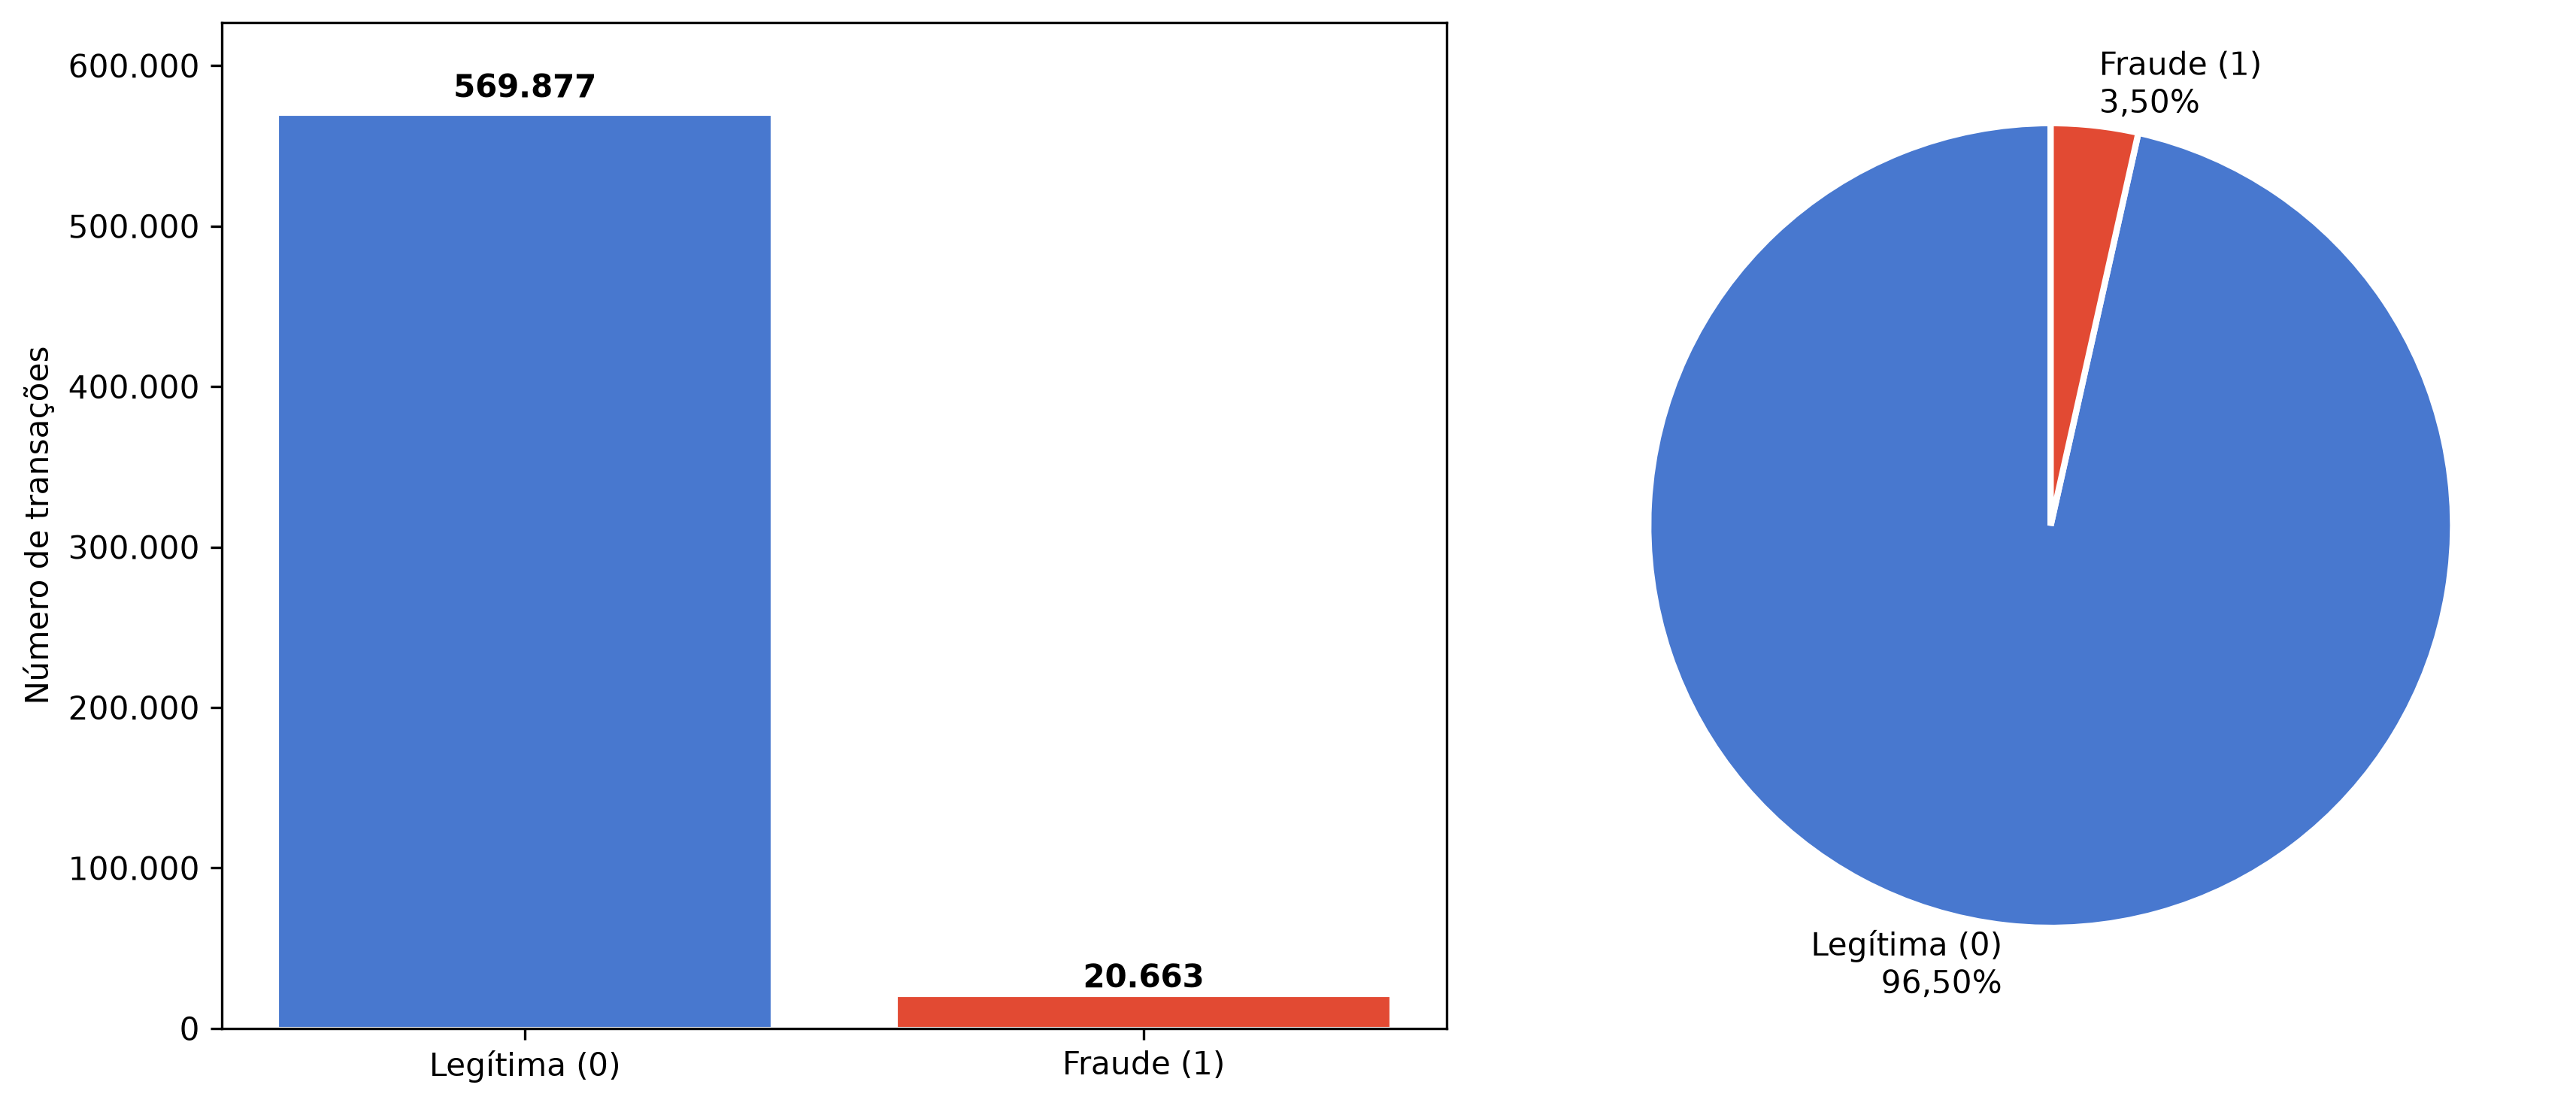
\includegraphics[width=\textwidth]{figuras/fig_distribuicao_alvo.png}
    \legend{Fonte: elaborada pelos autores (2026).}
\end{figure}

\section{Linha de base e efeito da divisão temporal}

A regressão logística, com o mesmo pré-processamento dos demais modelos, foi executada com ponderação de classe e com SMOTE aplicado somente ao treino \cite{chawla2002smote}. Na execução registrada em 06/09/2026, a AUC-PR de validação foi 0,3934 com ponderação de classe e 0,3967 com SMOTE, e a AUC-ROC foi 0,8414 e 0,8392. A diferença de 0,0033 na AUC-PR foi considerada empate, e a escolha foi decidida por critérios secundários, todos favoráveis à ponderação de classe: ela não cria transações sintéticas, não gera combinações inexistentes entre categorias já codificadas, como ocorre na interpolação do SMOTE após o \emph{one-hot encoding}, e não duplica o treino em memória. Essa mesma estratégia foi expressa no XGBoost final pelo parâmetro \texttt{scale\_pos\_weight}, fixado na razão real entre as classes do treino (27,43).

Para medir o efeito da forma de divisão, a mesma regressão logística com ponderação de classe foi avaliada em duas configurações na execução de 10/09/2026, apresentadas na Tabela~\ref{tab:divisao}. Os números dessa tabela pertencem a uma única execução e não são combinados com os da execução anterior, cujas casas decimais divergem ligeiramente por efeito do processamento em precisão simples.

\begin{table}[htb]
    \caption{Regressão logística com divisão temporal e com divisão aleatória estratificada}
    \label{tab:divisao}
    \centering
    \begin{tabular}{lcc}
        \hline
        Métrica & Divisão temporal & Divisão aleatória \\
        \hline
        AUC-PR na validação & 0,3936 & 0,4220 \\
        AUC-PR no teste & 0,1858 & 0,4250 \\
        Variação da validação para o teste & $-$52,8\% & +0,7\% \\
        AUC-ROC no teste & 0,8289 & 0,8604 \\
        \hline
    \end{tabular}
    \legend{Fonte: elaborada pelos autores (2026).}
\end{table}

Na divisão temporal, a AUC-PR caiu para menos da metade entre validação e teste, embora a taxa de fraude das duas partições fosse semelhante. Na divisão aleatória, validação e teste ficaram praticamente iguais, e a AUC-PR de teste foi 2,3 vezes maior. A divisão aleatória, portanto, descreveria um modelo estável e mais preciso do que o observado no período mais recente. Essa diferença, contudo, não pode ser atribuída apenas ao tempo: na divisão aleatória, transações de um mesmo identificador mascarado \texttt{card1} aparecem simultaneamente no treino e no teste. Separar os dois efeitos exigiria uma divisão por grupo, não executada. Por esse motivo, o fenômeno é descrito como degradação de desempenho no período posterior, e não como \emph{concept drift} comprovado.

\section{Comparação entre classificadores}

A Tabela~\ref{tab:modelos} compara os classificadores na validação. Todos usaram o mesmo pré-processamento, o mesmo corte temporal, a mesma estratégia de ponderação e o mesmo código de avaliação. A comparação utiliza AUC-PR e AUC-ROC, que independem do limiar de decisão.

\begin{table}[htb]
    \caption{Desempenho dos classificadores no conjunto de validação}
    \label{tab:modelos}
    \centering
    \begin{tabular}{lcc}
        \hline
        Modelo & AUC-PR & AUC-ROC \\
        \hline
        Regressão logística (linha de base) & 0,3934 & 0,8414 \\
        Random Forest, profundidade máxima 20 & 0,4573 & 0,8751 \\
        XGBoost, hiperparâmetros padrão & 0,5293 & 0,9044 \\
        Random Forest, árvores completas & 0,5298 & 0,9078 \\
        XGBoost ajustado (artefato entregue) & 0,5719 & 0,9067 \\
        \hline
    \end{tabular}
    \legend{Fonte: elaborada pelos autores (2026).}
\end{table}

Os modelos baseados em árvores superaram a linha de base com folga, o que justifica a complexidade adicional em relação a um modelo linear. Com hiperparâmetros padrão, porém, o XGBoost e o Random Forest com árvores completas ficaram empatados (0,5293 e 0,5298) \cite{chen2016xgboost,breiman2001random}. O XGBoost só se destacou após a busca de hiperparâmetros, que não foi aplicada ao Random Forest por seu papel de modelo comparativo. A evidência, portanto, não sustenta superioridade genérica do XGBoost: ela mostra que a configuração ajustada apresentou o melhor resultado entre as configurações avaliadas.

Limitar a profundidade do Random Forest a 20 reduziu o custo de treinamento, mas diminuiu a AUC-PR em 0,07. Com árvores completas, a floresta atingiu profundidade média de 64 níveis, e a média entre as 100 árvores aproveitou essa capacidade adicional.

\section{Ajuste do XGBoost e escolha do limiar}

A busca de hiperparâmetros do XGBoost otimizou a AUC-PR na validação em 50 tentativas, das quais 25 foram interrompidas antecipadamente por poda. Por viabilidade computacional, cada tentativa foi treinada com as 150 mil transações mais recentes do treino, e o espaço de busca limitou o modelo a 300 árvores e profundidade 8. A melhor configuração atingiu esses dois limites, de modo que não se afirma que seja um ótimo global. Retreinado no treino completo com os parâmetros selecionados, o modelo obteve AUC-PR de 0,5719 na validação e passou a ser o artefato entregue.

O limiar de decisão foi escolhido na validação pela maximização do F1, resultando em 0,6834, e foi persistido antes de qualquer previsão no teste. Nesse ponto, a validação apresentou precisão de 0,6680, \emph{recall} de 0,4829 e F1 de 0,5606. O conjunto de teste não foi utilizado em nenhuma etapa de ajuste ou seleção.

\section{Desempenho no conjunto de teste}

O teste foi executado uma única vez, sobre 88.581 transações do período mais recente, das quais 3.083 eram fraudes. A Tabela~\ref{tab:teste} compara os resultados com os da validação no mesmo limiar.

\begin{table}[htb]
    \caption{Desempenho do XGBoost entregue com o limiar de 0,6834}
    \label{tab:teste}
    \centering
    \begin{tabular}{lcc}
        \hline
        Métrica & Validação & Teste \\
        \hline
        AUC-PR & 0,5719 & 0,4833 \\
        AUC-ROC & 0,9067 & 0,8700 \\
        Precisão & 0,6680 & 0,5852 \\
        \emph{Recall} & 0,4829 & 0,4324 \\
        F1 & 0,5606 & 0,4973 \\
        \hline
    \end{tabular}
    \legend{Fonte: elaborada pelos autores (2026).}
\end{table}

A AUC-PR caiu 0,0887 entre validação e teste, repetindo, em menor intensidade, a degradação observada na linha de base. A Figura~\ref{fig:curvapr} mostra as curvas de precisão-\emph{recall} das duas partições e o ponto de operação correspondente ao limiar. No teste, a curva permanece muito acima da referência aleatória (0,0348), mas se desloca para baixo em toda a faixa de \emph{recall}.

\begin{figure}[htb]
    \caption{Curvas de precisão-\emph{recall} do XGBoost na validação e no teste}
    \label{fig:curvapr}
    \centering
    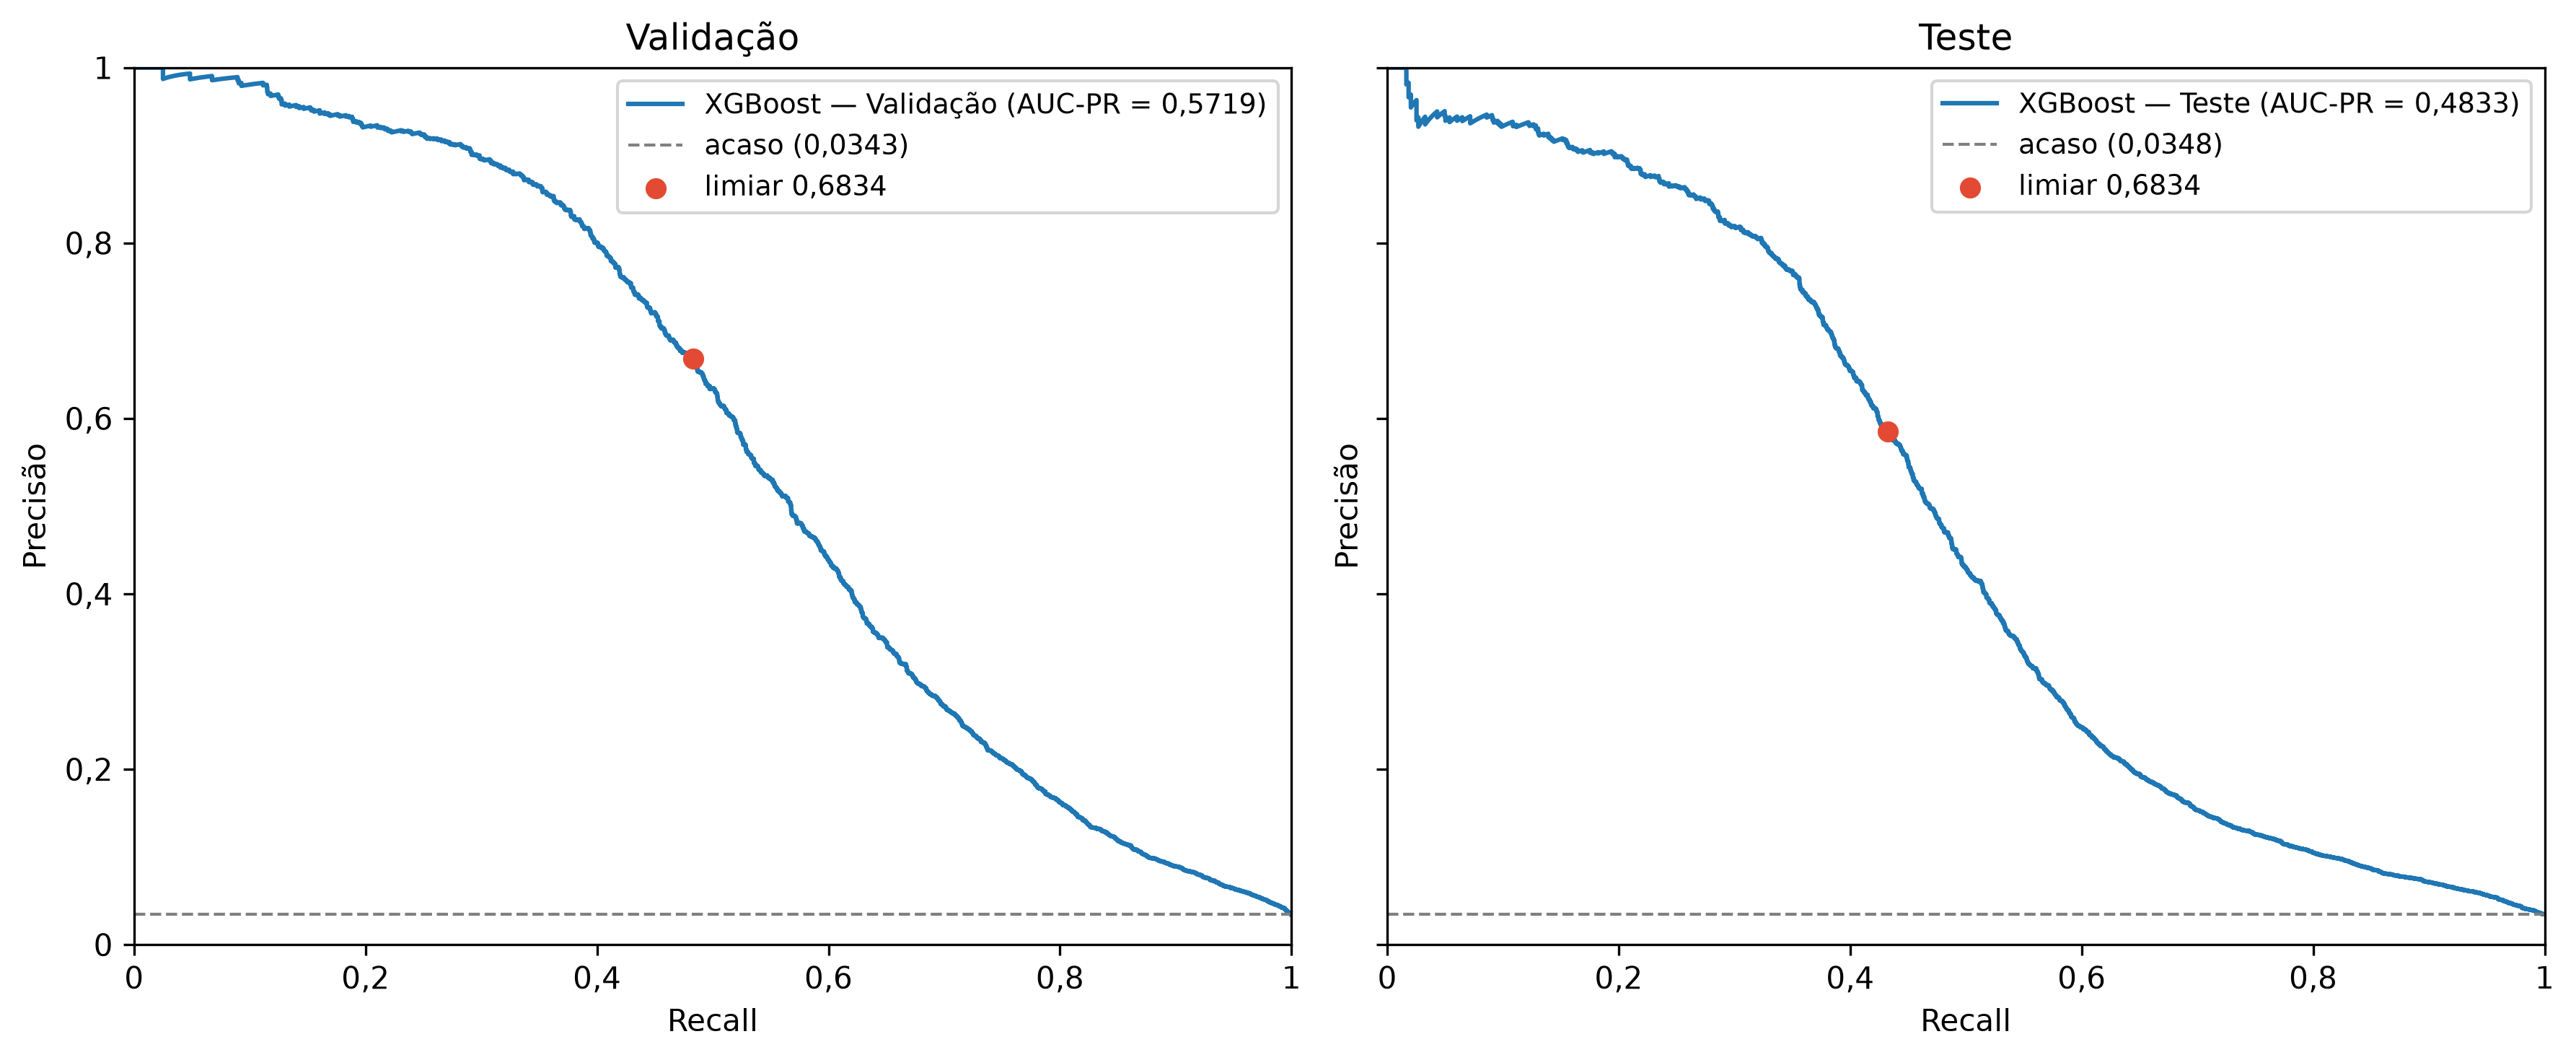
\includegraphics[width=\textwidth]{figuras/fig_curva_pr.png}
    \legend{Fonte: elaborada pelos autores (2026).}
\end{figure}

A matriz de confusão do teste é apresentada na Figura~\ref{fig:confusao}. O modelo sinalizou 2.278 transações, das quais 1.333 eram fraudes e 945 eram legítimas; outras 1.750 fraudes não foram detectadas. Em termos operacionais, cerca de seis em cada dez alertas corresponderam a fraudes rotuladas, enquanto pouco mais de quatro em cada dez fraudes foram recuperadas. O limiar escolhido levou, assim, a uma operação seletiva, que privilegia a precisão dos alertas em detrimento da cobertura.

\begin{figure}[htb]
    \caption{Matriz de confusão do XGBoost no conjunto de teste}
    \label{fig:confusao}
    \centering
    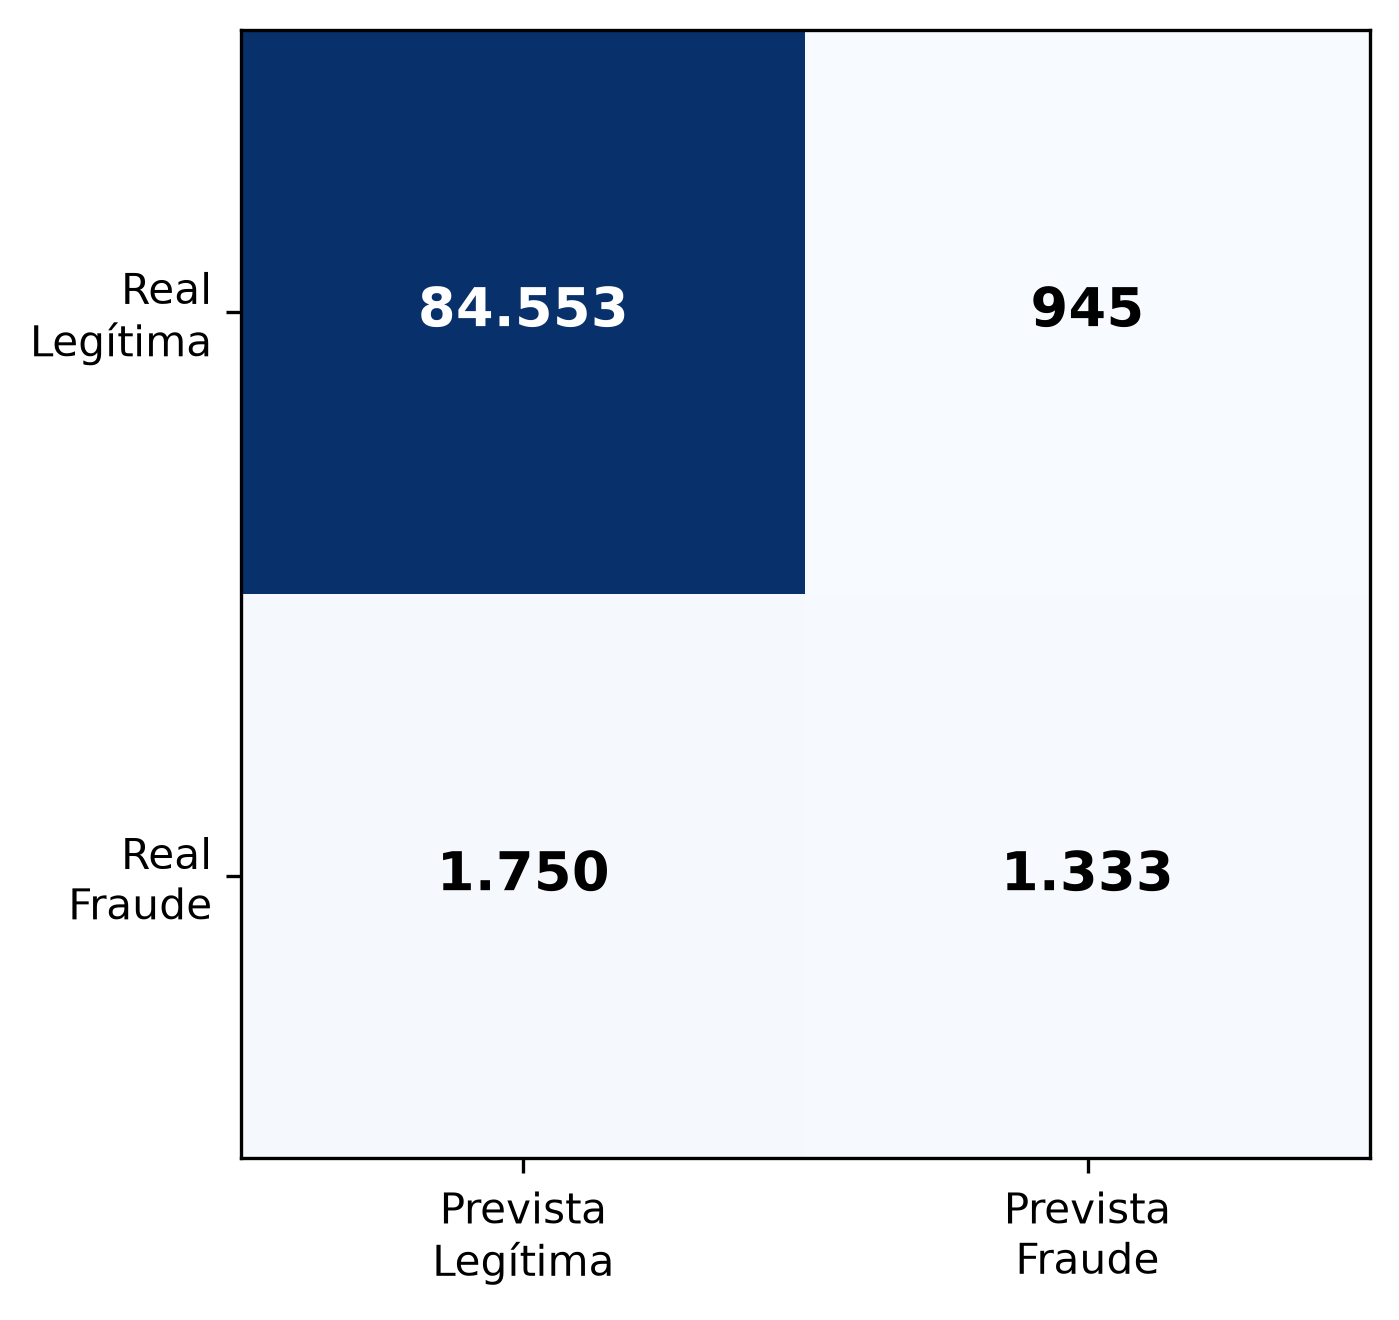
\includegraphics[width=0.55\textwidth]{figuras/fig_matriz_confusao_teste.png}
    \legend{Fonte: elaborada pelos autores (2026).}
\end{figure}

A AUC-ROC de 0,8700 indica boa capacidade de ordenação, mas a AUC-PR de 0,4833 descreve com mais clareza a dificuldade de recuperar fraudes sem gerar falsos alarmes. Com 3,48\% de fraudes no teste, o grande número de transações legítimas mantém a taxa de falsos positivos baixa mesmo com centenas de alertas incorretos, o que torna a AUC-ROC otimista nesse cenário \cite{saito2015precision}.

\section{Explicabilidade com SHAP}

A verificação de fidelidade aprovou todas as explicações: o maior erro na igualdade entre o valor-base somado às contribuições e a probabilidade prevista foi de aproximadamente $3{,}04 \times 10^{-7}$, abaixo da tolerância de $10^{-5}$ \cite{lundberg2017unified}. A Figura~\ref{fig:shapglobal} apresenta a importância global calculada sobre 1.000 transações da validação.

\begin{figure}[htb]
    \caption{Importância global SHAP do XGBoost na validação}
    \label{fig:shapglobal}
    \centering
    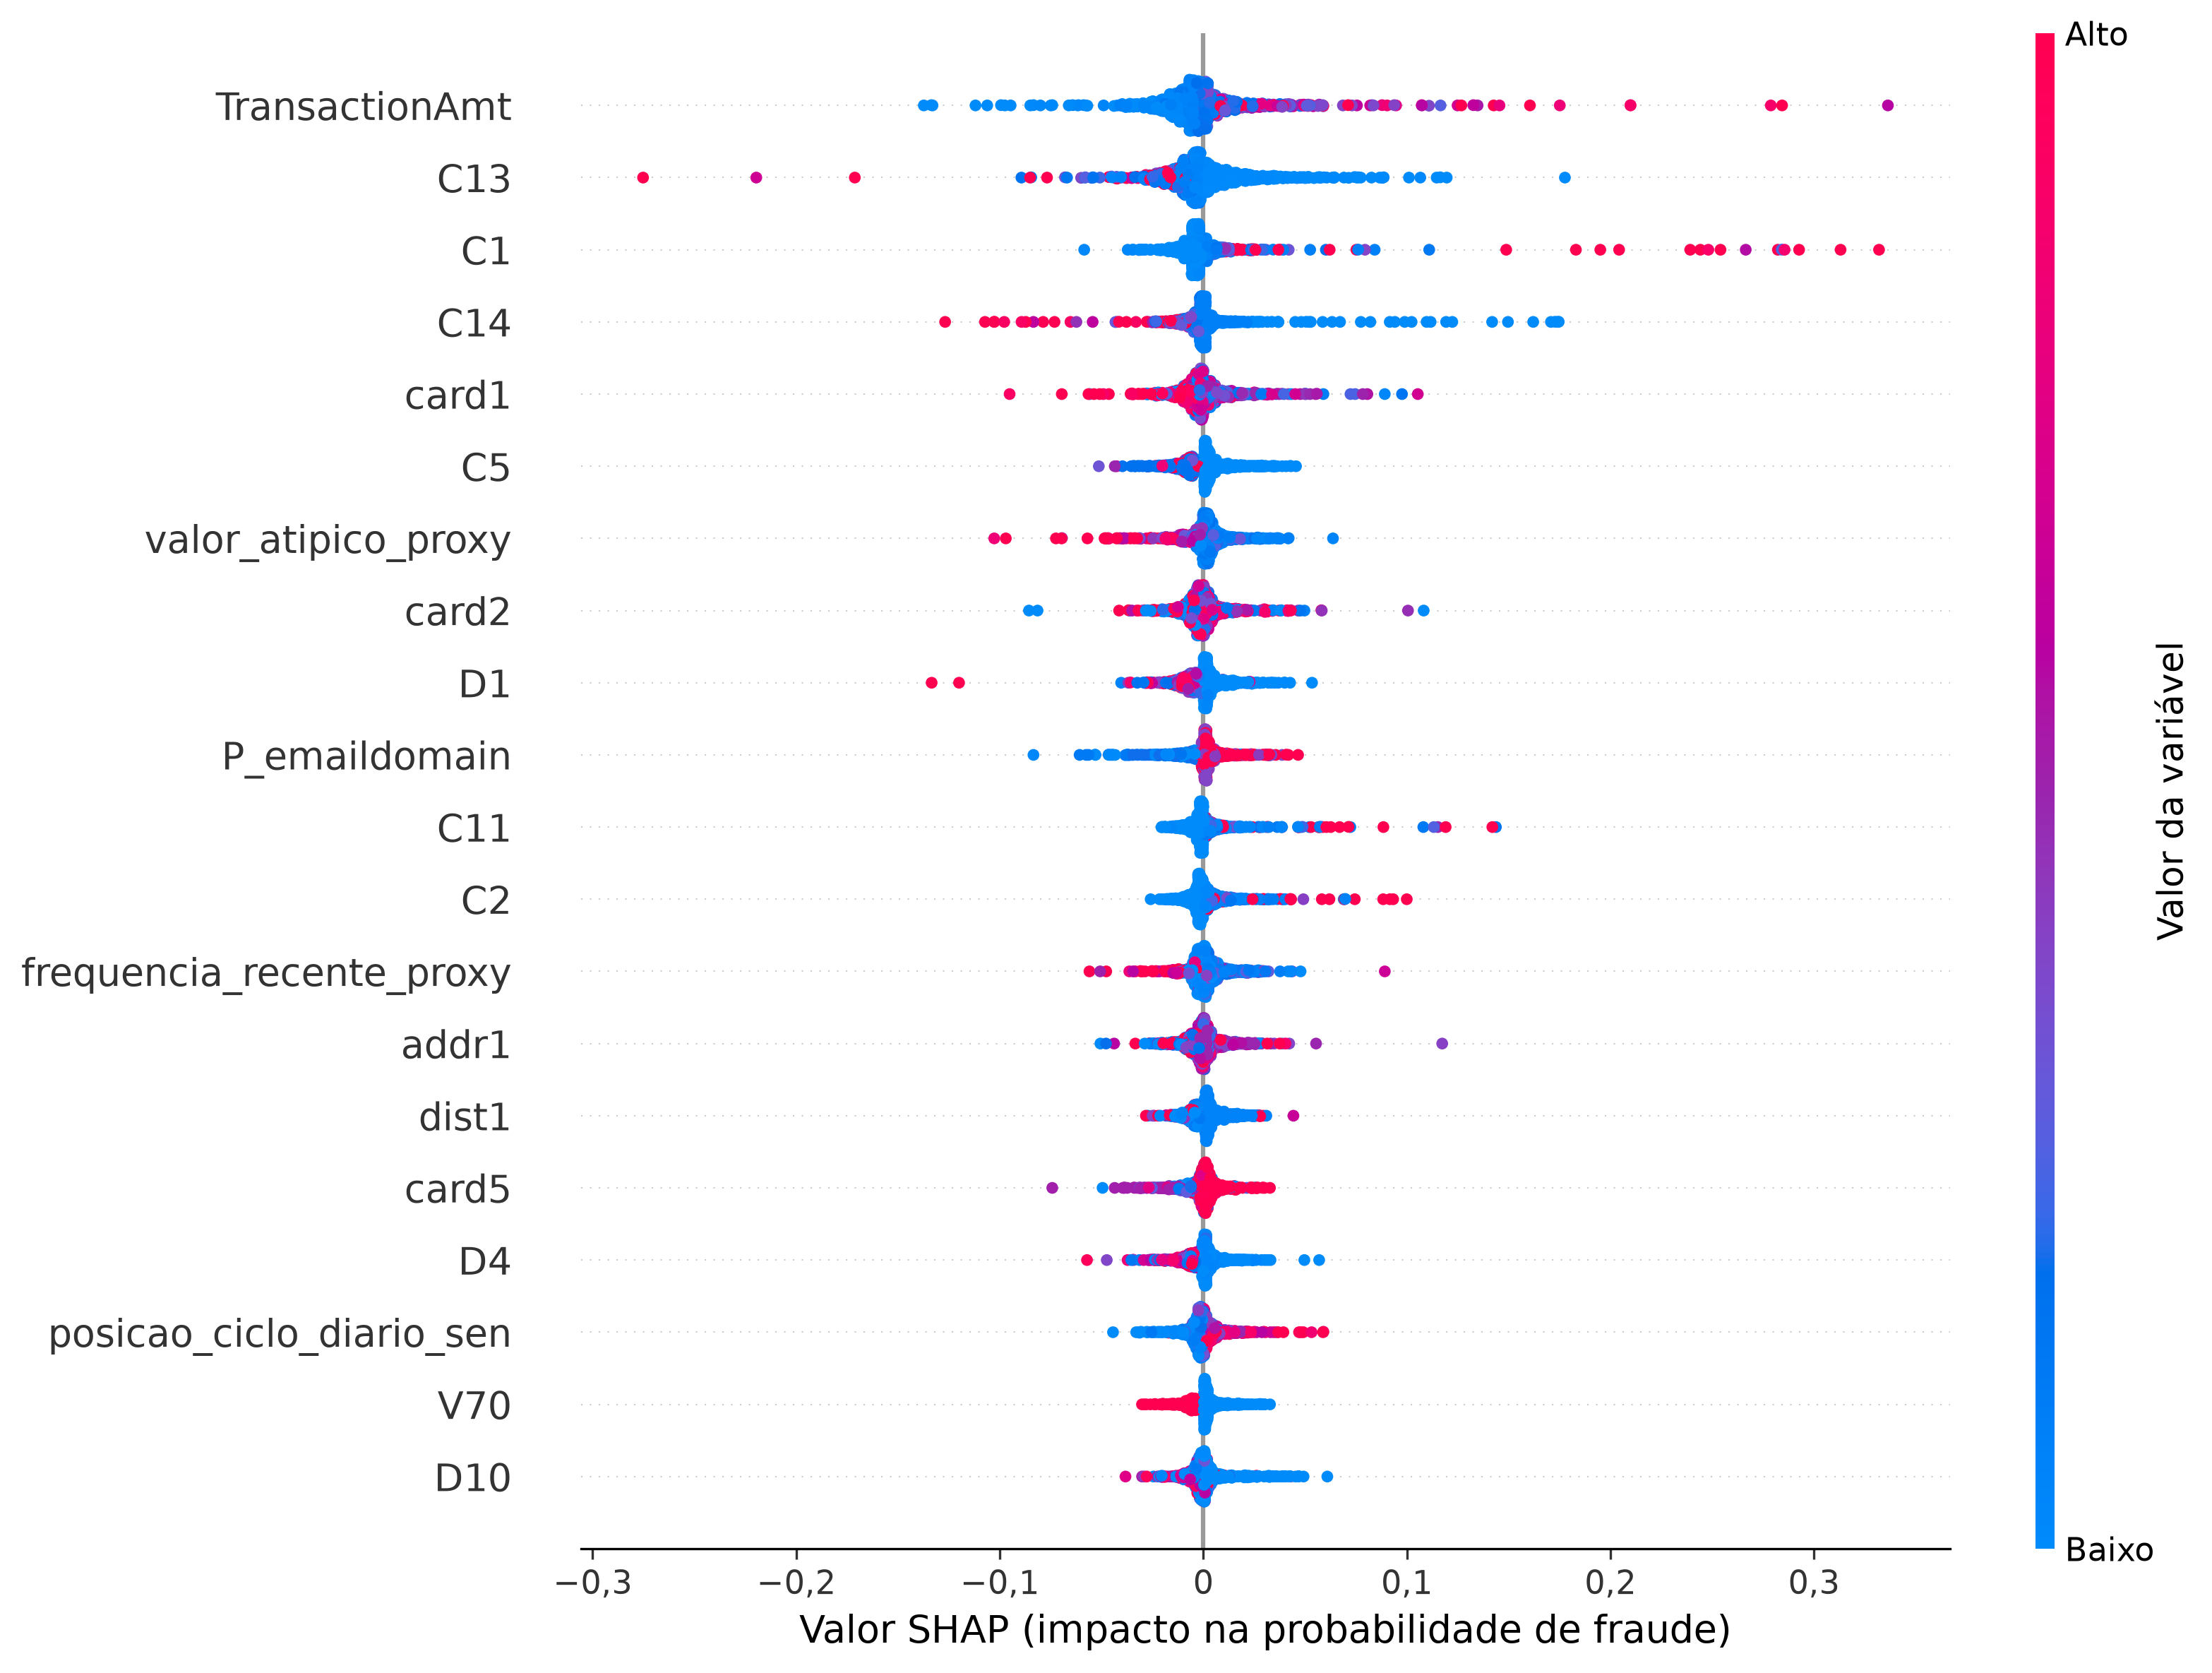
\includegraphics[width=0.9\textwidth]{figuras/fig_shap_summary.png}
    \legend{Fonte: elaborada pelos autores (2026).}
\end{figure}

As cinco variáveis de maior média absoluta de contribuição foram \texttt{TransactionAmt}, \texttt{C13}, \texttt{C1}, \texttt{C14} e \texttt{card1}. Entre as quatro proxies construídas no projeto, \texttt{valor\_atipico\_proxy} ocupou a 7ª posição e \texttt{frequencia\_recente\_proxy}, a 13ª, entre 460 variáveis após o pré-processamento. A posição cíclica no dia, representada pelas componentes seno e cosseno e pelo valor relativo, apareceu na 18ª, 23ª e 26ª posições. Já \texttt{dispositivo\_raro\_proxy} teve contribuição pequena, na 56ª posição. Duas das proxies com significado conhecido, portanto, tiveram participação relevante no comportamento do modelo, mas a maior parte das variáveis mais influentes continua sendo de colunas cujo significado foi mascarado na base original.

A Figura~\ref{fig:shapcasos} mostra as maiores contribuições em quatro casos da validação: um verdadeiro positivo, um falso positivo, um falso negativo e um verdadeiro negativo, escolhidos pela probabilidade mediana de cada quadrante. Esses casos foram selecionados com o limiar histórico de 0,5; as contribuições não dependem do limiar, mas a classificação de cada caso no ponto de operação final pode ser diferente.

\begin{figure}[htb]
    \caption{Contribuições SHAP em quatro casos da validação}
    \label{fig:shapcasos}
    \centering
    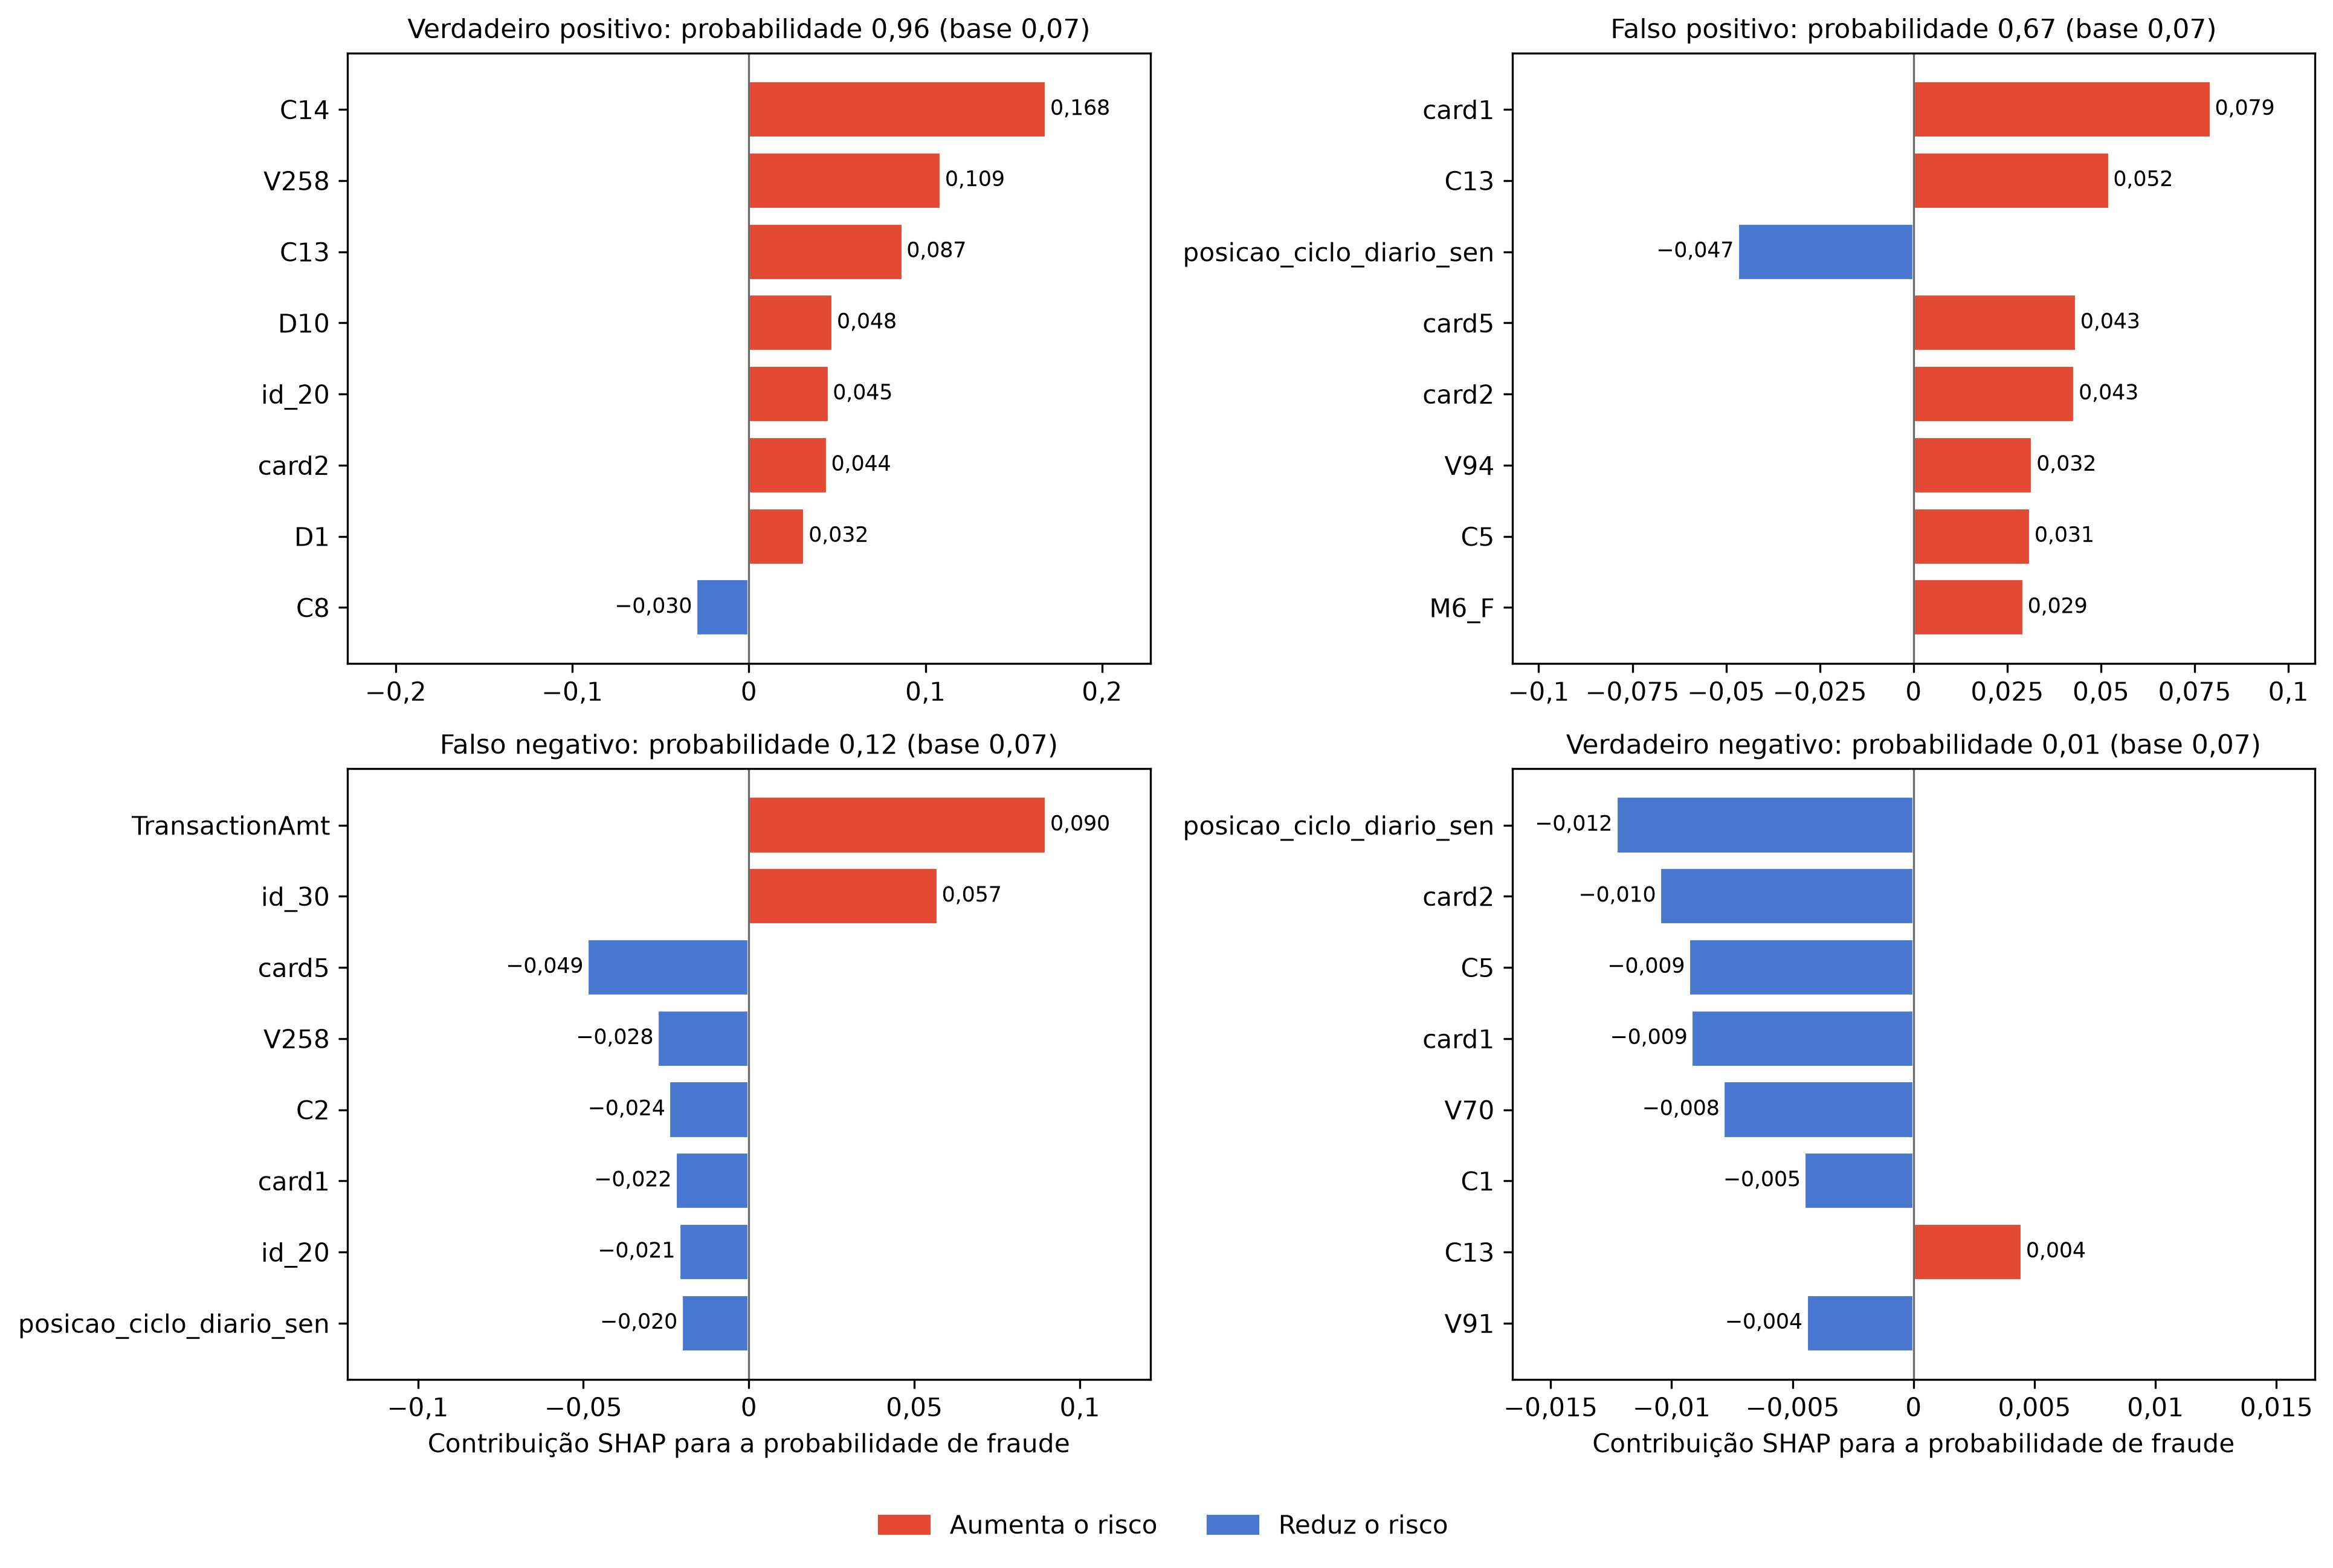
\includegraphics[width=\textwidth]{figuras/fig_shap_casos.png}
    \legend{Fonte: elaborada pelos autores (2026).}
\end{figure}

No verdadeiro positivo, com probabilidade de 0,96, as contribuições de \texttt{C14}, \texttt{V258} e \texttt{C13} somaram mais de 0,36 à probabilidade-base de 0,07. No falso positivo, \texttt{card1} e \texttt{C13} elevaram o risco a 0,67, apesar de a posição cíclica no dia ter atuado na direção contrária. No falso negativo, o valor da transação aumentou o risco, mas não o suficiente para compensar as contribuições negativas de outras variáveis, e a probabilidade ficou em 0,12. Esses exemplos ilustram o uso do SHAP como instrumento de auditoria: ele mostra quais variáveis sustentaram cada previsão, inclusive nos erros, mas descreve influência sobre o modelo, e não causalidade ou culpa.

\section{Camada documental e integração}

A base vetorial reconstruída em 20/09/2026 reuniu quatro fontes, 290 \emph{chunks} pais e 1.195 vetores de 384 dimensões em um índice FAISS exato \cite{johnson2021billion,reimers2019sentencebert}. As consultas de fumaça recuperaram trechos relacionados ao Mecanismo Especial de Devolução e ao Guia do MED, demonstrando que o índice pode ser carregado e consultado. Essas consultas verificam o funcionamento técnico, mas não medem relevância.

Durante a integração, observou-se que consultas formadas pelos nomes das variáveis de maior contribuição SHAP, em sua maioria anonimizadas, como \texttt{C13} ou \texttt{V258}, não oferecem termos com significado textual para a busca semântica. Por isso, a versão atual do pipeline restringe a camada de explicação às quatro proxies documentadas no projeto: somente elas compõem a consulta ao índice, o contexto enviado ao modelo de linguagem e o painel SHAP da interface. O classificador continua utilizando todas as variáveis. A restrição impede que colunas anônimas recebam significado inventado, mas implica que a explicação apresentada não corresponde necessariamente às maiores contribuições do modelo para aquela transação.

O pipeline carrega o modelo, o pré-processador e o limiar de 0,6834 persistido na política de decisão, de modo que a interface opera no mesmo ponto avaliado no teste. O cliente para o modelo de linguagem Claude Haiku 4.5 foi implementado com tratamento de falhas: na ausência de credencial ou em caso de erro, a interface não gera explicação substituta e mantém visíveis a classificação, os fatores SHAP e os documentos recuperados \cite{lewis2020rag}. Até o fechamento desta versão, entretanto, não foram registradas explicações geradas pelo modelo de linguagem, e o protocolo de avaliação de recuperação e geração não foi executado \cite{es2024ragas}. Os resultados de relevância dos documentos, coerência com o SHAP, fidelidade aos dados, alucinação e clareza permanecem \texttt{\{\{RESULTADO\}\}}.

\section{Discussão}

Os resultados indicam que a combinação de um classificador baseado em árvores com explicações SHAP é tecnicamente viável no conjunto estudado. O XGBoost ajustado superou a linha de base com margem ampla e manteve, no teste, uma AUC-PR cerca de 14 vezes maior que a de um classificador aleatório. A explicação local foi numericamente fiel ao modelo e permitiu examinar tanto acertos quanto erros.

Três ressalvas delimitam essas conclusões. A primeira é a degradação no período posterior, presente tanto na linha de base quanto no modelo final, que reforça a necessidade de avaliação temporal e de revalidação periódica antes de qualquer uso. A segunda é a assimetria na comparação entre modelos: como apenas o XGBoost passou por busca de hiperparâmetros, não é possível afirmar que ele seja superior ao Random Forest. A terceira é a natureza da base: o IEEE-CIS representa transações de comércio eletrônico com cartão, e as proxies inspiradas no Pix são aproximações experimentais. Tipos de chave, perfil do destinatário, idade da conta e outros elementos do arranjo Pix não estão representados.

A anonimização das variáveis também conecta as limitações da segunda e da terceira camadas. Ela restringe a interpretação dos valores SHAP e, pelo mesmo motivo, oferece poucos termos úteis para a recuperação documental. A priorização das proxies com significado conhecido foi a alternativa adotada para que as consultas usem conceitos como valor atípico ou frequência recente, em vez de códigos sem interpretação direta. A contribuição da camada RAG, contudo, só poderá ser estabelecida após a execução do protocolo de avaliação com respostas reais do modelo de linguagem.
